\documentclass{article}
\usepackage[utf8]{inputenc}
\usepackage[spanish]{babel}
\usepackage{listings}
\usepackage{graphicx}
\usepackage{hyperref}
\graphicspath{ {images/} }
\usepackage{cite}

\begin{document}

\begin{titlepage}
    \begin{center}
        \vspace*{1cm}
            
        \Huge
        \textbf{Manual de usuario - Informatica II.}
            
        \vspace{0.5cm}
        \LARGE
            
        \vspace{1.5cm}
            
        \textbf{Luis Miguel Gil Rodriguez.}
        \\
        \textbf{Maverick Sossa Tobon.}
        \vfill
        \vspace{0.8cm}
            
        \Large
        Despartamento de Ingeniería Electrónica y Telecomunicaciones\\
        Universidad de Antioquia\\
        Medellín\\
        Septiembre de 2021
            
    \end{center}
\end{titlepage}
\tableofcontents
\newpage
\section{Manual de usuario.} \label{intro}
En este corto pero eficiente manual de usuario podrás aprender cómo utilizar nuestro software para mostrar una bandera en una matriz de 16X16 LEDs, como lo mostraremos en los siguientes ejemplos:
\begin{figure}[h]
  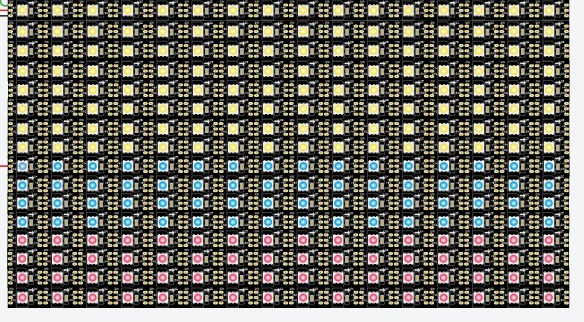
\includegraphics[width=10cm]{Colombia.jpg}
  \centering
  \caption{La bandera de Colombia en la matriz de LEDs.}
  \label{fig:Colombia}
\end{figure}
\begin{figure}[h]
  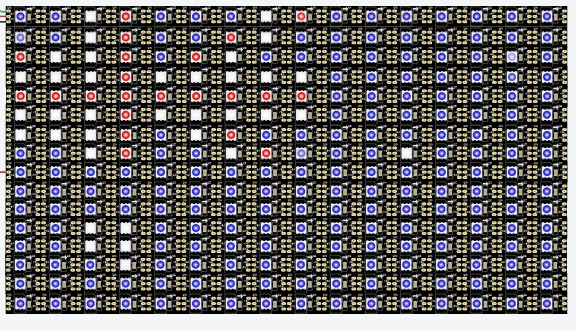
\includegraphics[width=10cm]{Australia.jpg}
  \centering
  \caption{La bandera de Australia en la matriz de LEDs.}
  \label{fig:Colombia}
\end{figure}
\subsection{En Qt.}
Cuando tenga descargado o clonado en su computador el repositorio \url{https://github.com/MiguelGil1/Parcial_ll_Info_ll}, deberá ir a la carpeta Codigo-fuente y luego a la carpeta del proyecto de Qt, el cual se llama Algorithm-Resize-Img y darle doble click al archivo Algorithm-Resize-Img.pro.
\begin{figure}[h]
  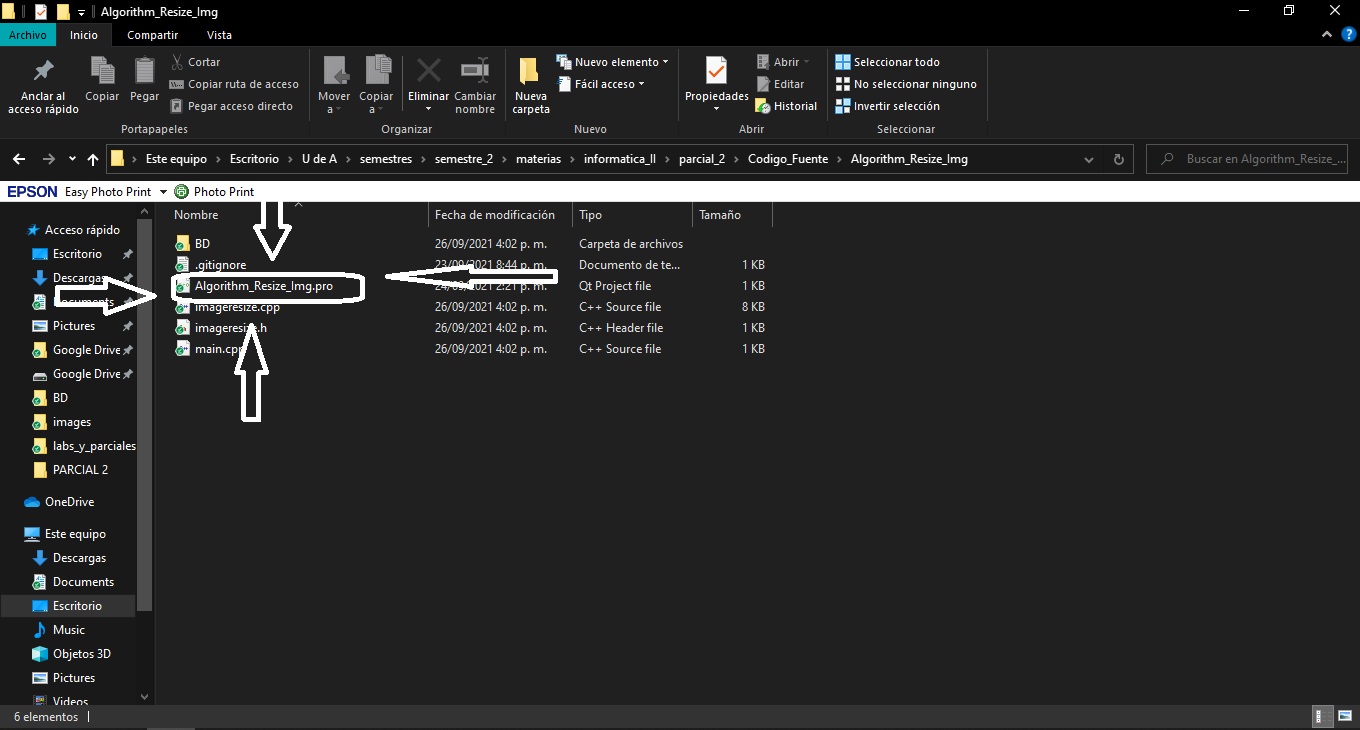
\includegraphics[width=10cm]{explorador_archivos.PNG}
  \centering
  \caption{Explorador de archivos}
  \label{fig:explorador_archivos}
\end{figure}
Al hacer este paso, se abrirá de inmediatamente Qt y te preguntara que con que kit desea construir el proyecto, como se muestra a continuación:
\begin{figure}[h]
  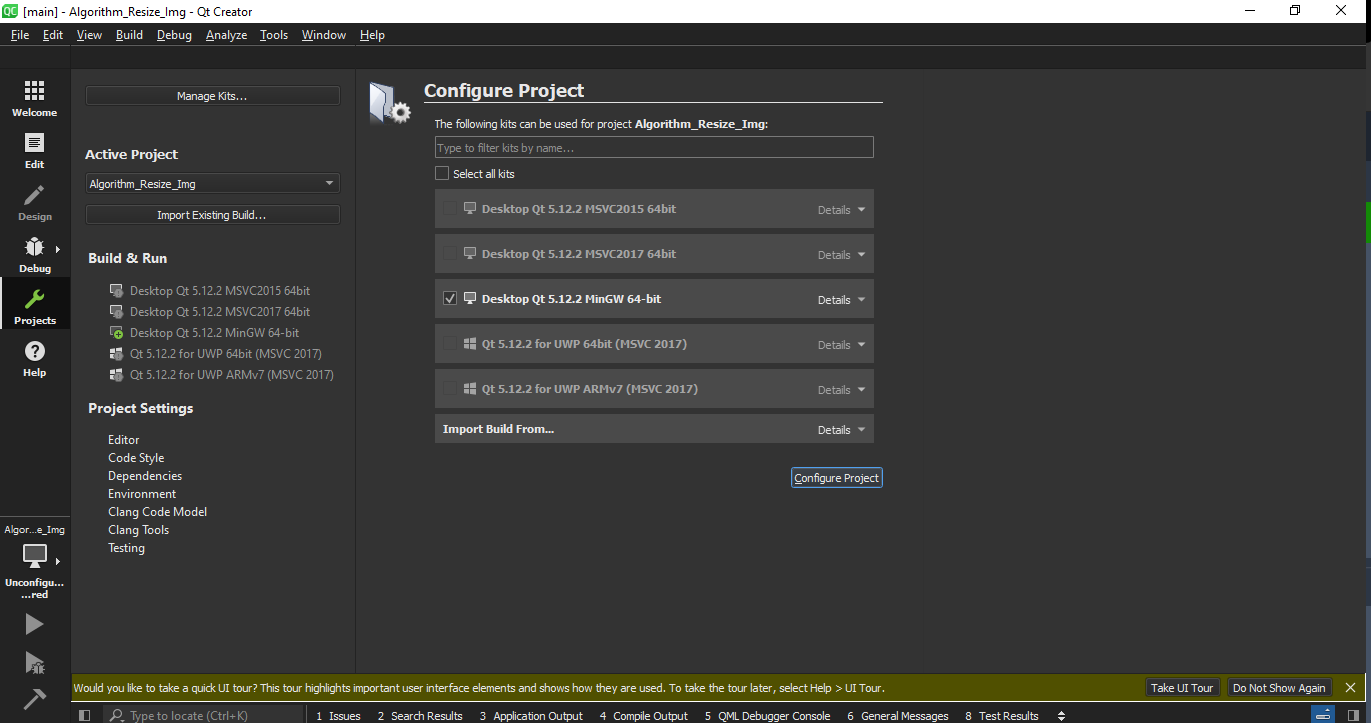
\includegraphics[width=10cm]{build.PNG}
  \centering
  \caption{Seleccion de Kit de construccion.}
  \label{fig:build}
\end{figure}
Selecciona el de kit de confianza y presionas el botón “Configure Project”:
\\
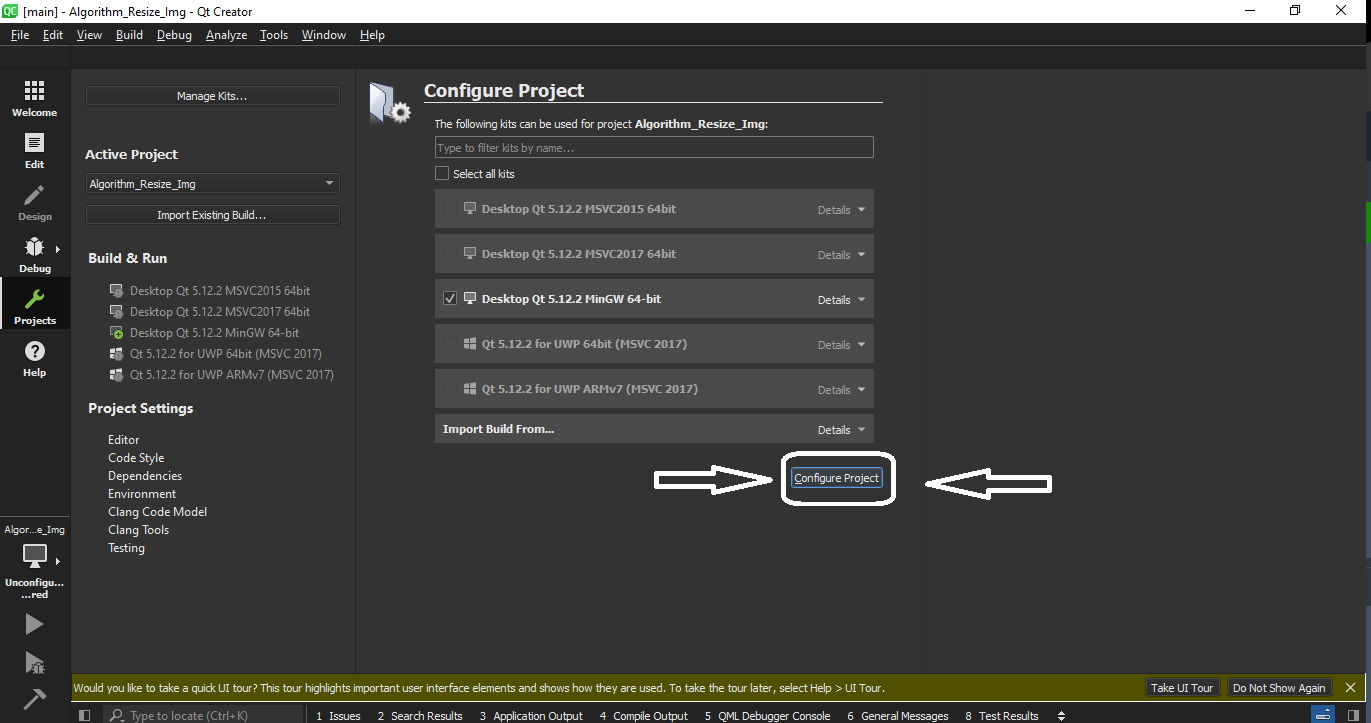
\includegraphics[width=10cm]{configurar_proyecto.PNG}
\\
Cuando el proyecto termine de cargar y configurar, presione el Botón “Run” para ejecutar el programa:
\begin{figure}[h]
  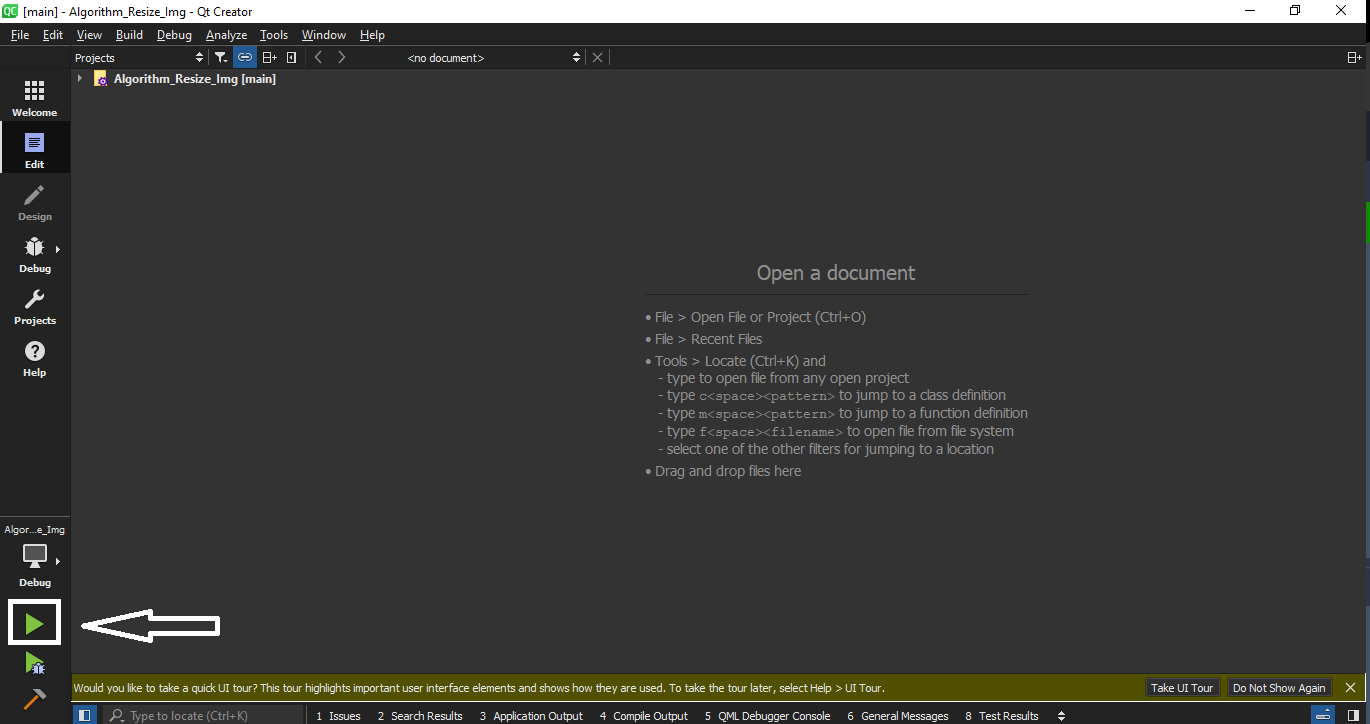
\includegraphics[width=10cm]{run.PNG}
  \centering
  \caption{Boton "Run".}
  \label{fig:run}
\end{figure}
\subsection{En Tinkercad.}
Luego de haber ejecutado satisfactoriamente el programa de redimensionamiento de Imágenes, iremos a la Carpeta DB, ubicada dentro del proyecto de Qt, en la cual podemos encontrar archivo de texto titulado “ImgResize.txt”, allí podremos encontrar la información de la imagen redimensionada dividida en 3 matrices unidimensionales, las cuales representara la intensidad del Rojo, Verde o Azul en números enteros de 0 a 255
\\
Después de esto, procedemos a abrir el proyecto de Tinkercad, presionaremos el Botón “Código”, ubicado en la parte superior derecha de la pagina.
\begin{figure}[h]
  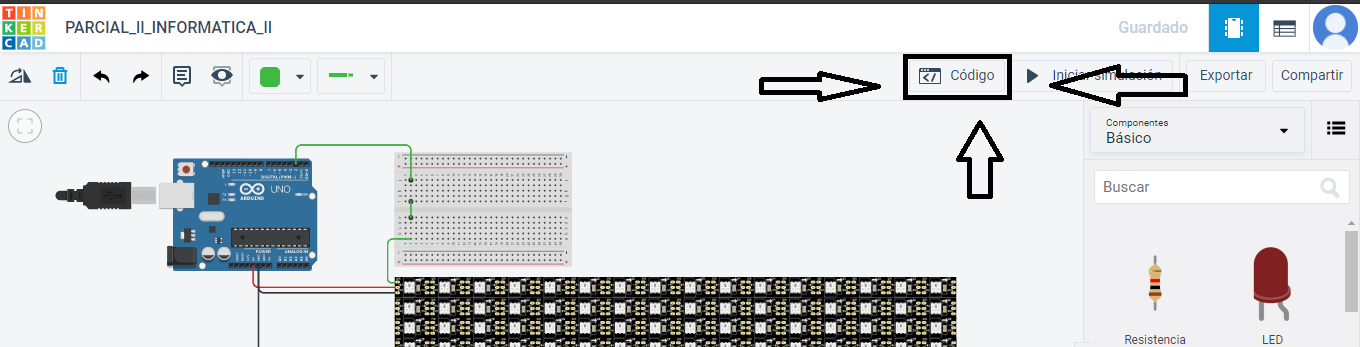
\includegraphics[width=10cm]{codigo.PNG}
  \centering
  \caption{Boton "Código".}
  \label{fig:Codigo}
\end{figure}
Procederemos a pegar la información del archivo “ImgResize.txt” en la línea número 19, de lo contrario el programa no funcionara de forma correcta, como e muestra en la siguiente imagen:
\begin{figure}[h]
  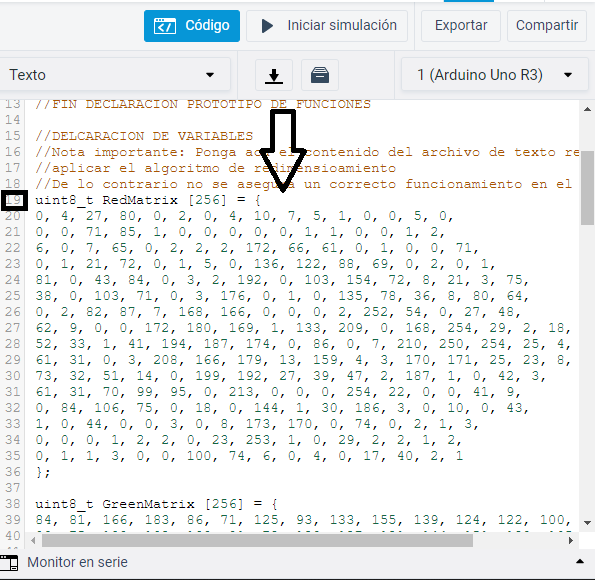
\includegraphics[width=10cm]{matrices.PNG}
  \centering
  \caption{Matrices del archivo en el Código.}
  \label{fig:matrices}
\end{figure}
Luego de esto, podemos presionar en el botón “Iniciar simulación”, el cual se encuentra al lado derecho del botón “Código”.
\begin{figure}[h]
  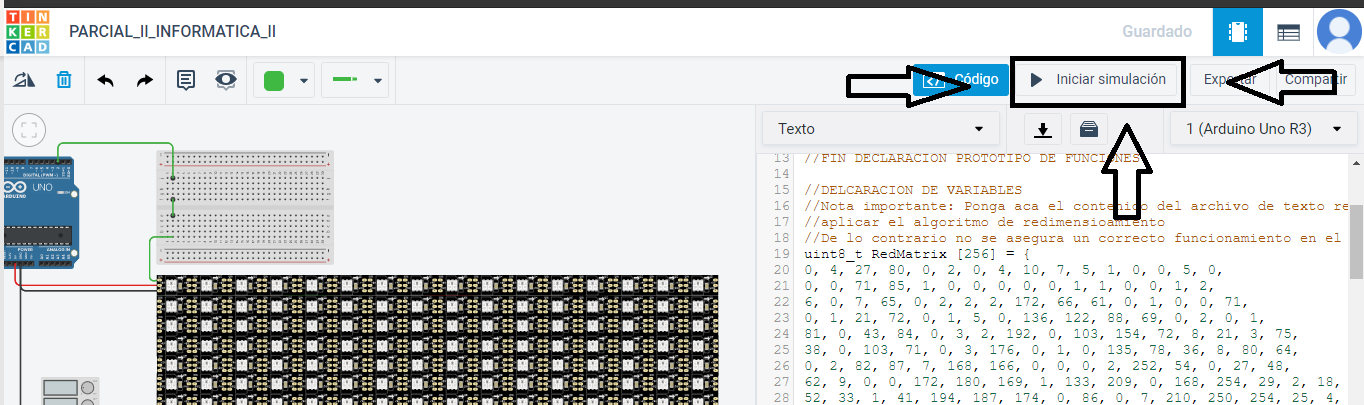
\includegraphics[width=10cm]{iniciar_simulacion.PNG}
  \centering
  \caption{Botón "Iniciar simulación".}
  \label{fig:iniciar_simulacion}
\end{figure}
Si desea evidenciar el valor que se le esta asignando a cada Píxel, puede dar un click en el Monitor Serial de Tinkercad, el cual se encuentra en la parte inferior del Código.
\begin{figure}[h]
  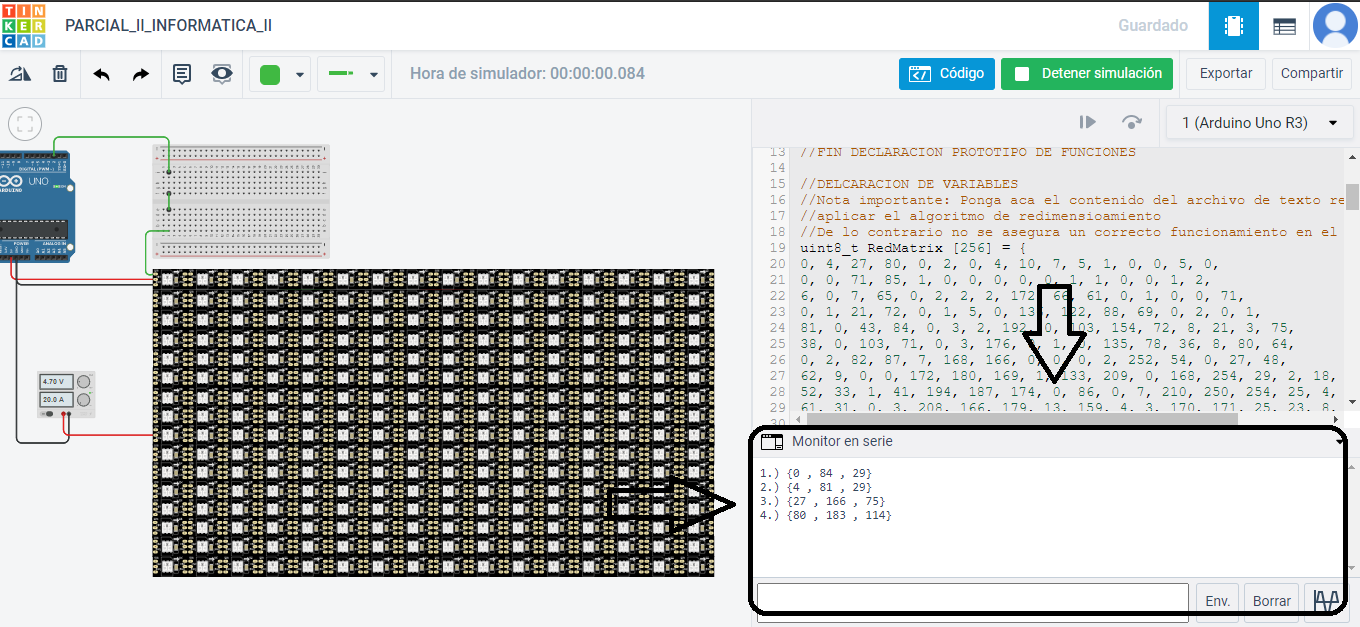
\includegraphics[width=10cm]{monitor_serial.PNG}
  \centering
  \caption{Monitor serial.}
  \label{fig:monitor_serial}
\end{figure}
Debe esperar hasta que el software envíe la información a cada LED de la matriz, una vez este proceso termine, inmediatamente se verá reflejado el resultado en la matriz como se muestra a continuación:
\begin{figure}[h]
  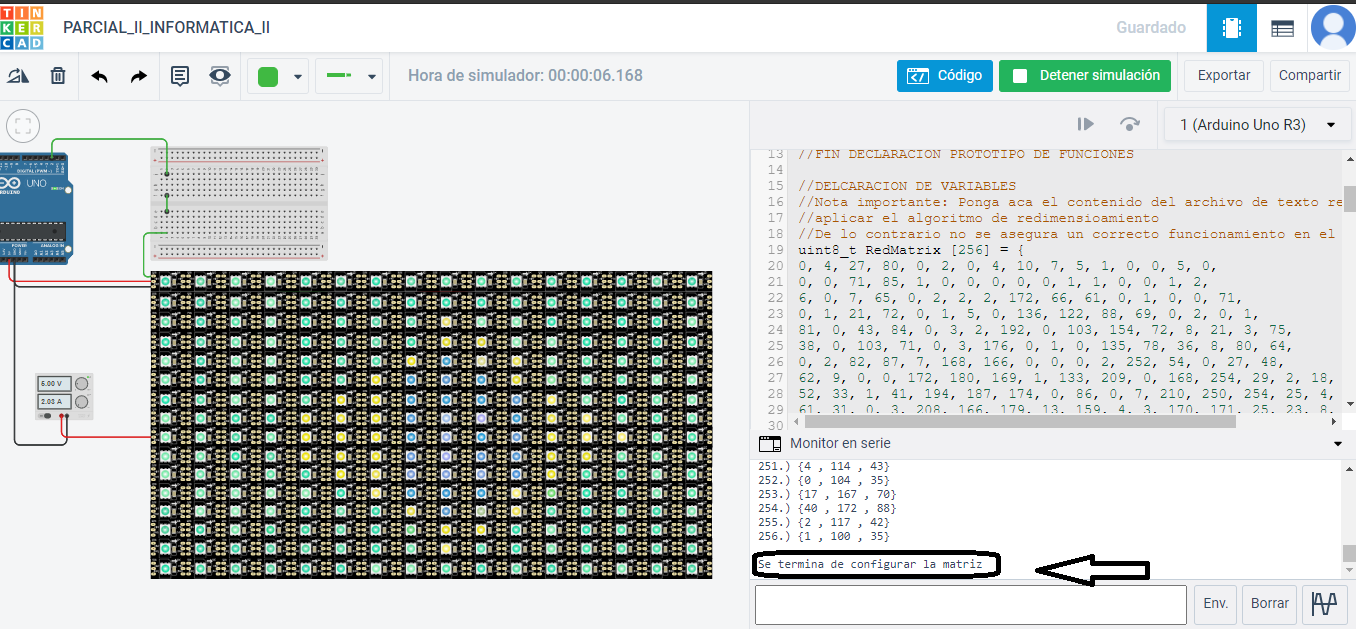
\includegraphics[width=10cm]{resultado.PNG}
  \centering
  \caption{Resultado (Bandera de Brasil).}
  \label{fig:Resultado}
\end{figure}
\bibliographystyle{IEEEtran}
\bibliography{references}
\end{document}
